\documentclass[11pt]{article}
\usepackage[T1]{fontenc}
\usepackage{lmodern,amsmath,amssymb}
\usepackage[margin=25mm]{geometry}
\usepackage{graphicx,float}
\usepackage{longtable,booktabs,array}
\usepackage{xcolor}
\usepackage[unicode]{hyperref}
\usepackage{xurl}
\hypersetup{pdfauthor={Eduardo Arana},pdftitle={Shared UI State and Host
Enforcement: A Bounded Case Study of Three Agent-UI
Configurations},colorlinks=true,allcolors=black}
\urlstyle{same}
\setcounter{secnumdepth}{3}
\setlength{\parindent}{1em}
\setlength{\parskip}{2pt}
\setlength{\emergencystretch}{3em}
\setlength{\LTpre}{6pt}
\setlength{\LTpost}{6pt}
\newcounter{none}
\providecommand{\tightlist}{\setlength{\itemsep}{0pt}\setlength{\parskip}{0pt}}
\newcommand{\pandocbounded}[1]{#1}
\renewcommand{\topfraction}{0.9}
\renewcommand{\bottomfraction}{0.8}
\renewcommand{\textfraction}{0.05}
\renewcommand{\floatpagefraction}{0.85}
\title{Shared UI State and Host Enforcement: A Bounded Case Study of
Three Agent-UI Configurations}
\author{Eduardo Arana}
\date{Arananet\\[4pt]21 September 2026 --- local draft; human review
pending}
\begin{document}
\special{pdf:minorversion 7}
\maketitle
\section*{Abstract}\label{abstract}

Agent-facing UI libraries and protocols provide different ways to
describe, host, and interact with interfaces. Comparing them requires
separating the format from the adapter and the host that implements it.
We examine an existing deterministic TypeScript harness using
json-render, A2UI, and MCP Apps in three scenarios: surface handoff,
fixed-order identifier collision, and action round-trip. The
shared-state configurations retain two handoff blocks in one surface and
replace an earlier summary when a later writer uses the same identifier.
The MCP Apps configuration allocates separate instances and retains both
summaries. Its model-only tool rejection depends on an explicitly
installed host handler; the existing permissive variant forwards the
call. These observations concern the tested configurations, not
intrinsic rankings of protocols. We map claims to source, assertions,
and execution evidence, distinguish retained artifacts from fresh
reruns, and identify confounders and missing checks. The local protocol
suite passed 24 tests; fresh browser execution was blocked by an
environment failure documented with the artifacts. This is a
retrospective engineering case study, with no LLM experiment,
performance measurement, or independent-person reproduction. Human
review remains pending.

\section{Introduction}\label{introduction}

A UI description, an execution environment, and an authorization
decision operate at different layers. Treating them as interchangeable
can make a comparison attribute a host policy to a wire format, or
attribute a namespace decision to a universal limitation. The practical
question is what the current configurations do when more than one named
writer contributes to a conceptual interface.

The contribution is an auditable interpretation of a small existing
harness. We provide an explicit scope, a falsifiable hypothesis, a
claim-to-check mapping, and a reproduction procedure. We do not claim
exhaustive novelty, replication of a prior study, an impossibility
proof, a fundamental tradeoff, or a universal protocol ranking. The
retained comparison report is an input to audit, not a scientific
oracle. Its broader wording and historical scenario names remain
unchanged; the bounds in this manuscript govern our conclusions.

\section{Research questions}\label{research-questions}

RQ1: Where do the existing adapters place the output of a scripted
surface handoff?

RQ2: What survives a fixed-order identifier-collision probe in the
configured namespaces?

RQ3: Which local bookkeeping and host decisions determine action routing
and model-only tool rejection?

\section{Methodology}\label{methodology}

This retrospective case study examines deterministic scripted agents,
with no LLM experiment. The unit of comparison is an SDK/adapter/host
configuration. Identical scenario input does not isolate protocol
causality. Three scenarios exercise three configurations, with an
existing permissive-host variant for MCP Apps in S3.

\subsection{A falsifiable local
hypothesis}\label{a-falsifiable-local-hypothesis}

H1: In S2, the fixed-order writes to the shared \texttt{summary} ID
leave the finance headline in the json-render and A2UI configurations,
while the MCP Apps configuration retains both headlines in separate
instances. A snapshot or DOM assertion showing the risk headline instead
of finance in a shared summary, or loss of either isolated headline,
would contradict this hypothesis for the tested configuration.

The \href{../src/scenarios/s2-concurrent-composition.ts}{S2 script}
awaits each emission: risk detail, finance detail, risk summary, then
finance summary. This is a fixed-order identifier-collision probe, not
actual concurrency or a scheduling benchmark. The historical filename
and test descriptions retain the word ``concurrent''. The focused check
uses the \href{../tests/protocol/scenarios.test.ts}{existing snapshot
assertions} and \href{../tests/browser/render.spec.ts}{browser
assertions}, rather than treating the adapter's \texttt{LOST} or
\texttt{ENFORCED} labels as measurements. Fresh execution status is
recorded separately from this source-based hypothesis.

\subsection{Configurations and
versions}\label{configurations-and-versions}

The \href{../package.json}{manifest} specifies ranges. The
\href{../package-lock.json}{lockfile} and locally installed package
metadata agree on the exact versions below. Package versions are not
protocol schema versions. These are observations of this checkout, not
recommendations or statements about the newest available releases.

{\def\LTcaptype{none} % do not increment counter
\begin{longtable}[]{@{}lll@{}}
\toprule\noalign{}
Configuration & Manifest range & Lockfile and installed version \\
\midrule\noalign{}
\endhead
\bottomrule\noalign{}
\endlastfoot
json-render core and React renderer & \texttt{\^{}0.21.0} each &
\texttt{0.21.0} each \\
A2UI web core and Lit renderer & \texttt{\^{}0.11.0} each &
\texttt{0.11.0} each \\
MCP Apps extension SDK & \texttt{\^{}2.0.0} & \texttt{2.0.0} \\
MCP client, core, and server & \texttt{\^{}2.0.0} each & \texttt{2.0.0}
each \\
React and React DOM & \texttt{\^{}19.2.3} each & \texttt{19.3.0} each \\
Lit & \texttt{\^{}3.3.3} & \texttt{3.3.3} \\
Zod & \texttt{\^{}4.2.0} & \texttt{4.6.5} \\
\end{longtable}
}

The A2UI adapter imports \texttt{@a2ui/web\_core/v0\_9} and emits
\texttt{version:\ "v0.9"}. Its package version \texttt{0.11.0} does not
mean that the experiment uses a v0.11 protocol. MCP Apps SDK
\texttt{2.0.0} likewise does not establish a wire protocol version. The
extension specification and SDK are separate references; no exact
upstream specification commit or negotiated wire-version value was
retained for this paper. Live repository documentation was inspected on
21 September 2026 and may differ from release-time documentation. The
local lockfile fixes the tested package resolution, not the mutable web
references.

The \href{../src/adapters/json-render/adapter.ts}{json-render adapter}
maintains one \texttt{Spec} per conceptual surface and maps logical
block, row, and control IDs to element keys. It calls
\texttt{applySpecPatch} for element additions/replacements and also
directly updates root children. Therefore, its patch log does not
capture every mutation. Its catalog validates emitted specs;
\texttt{writtenBy} is an ordinary catalog prop and \texttt{lastWriter}
is adapter bookkeeping. Neither is authenticated provenance.

The \href{../src/adapters/a2ui/adapter.ts}{A2UI adapter} validates
messages using \texttt{A2uiMessageSchema} and drives
\texttt{MessageProcessor}. Its component IDs and data paths derive from
block IDs. A shared \texttt{rootChildren} collection coordinates the
surface root. Node uses a schema-only harness catalog; the browser uses
the Lit basic catalog. Snapshot titles and writer names partly come from
adapter maps, while row values come from the data model. Surface
addressing is not authorization: an address identifies a target but does
not establish a caller's permission.

The \href{../src/adapters/mcp-apps/adapter.ts}{MCP Apps adapter} creates
one server per agent and one app instance per surface/agent pair. Its
Node path uses real SDK clients, servers, apps, and bridges connected by
in-memory transports. Its snapshot is reconstructed from adapter-held
blocks, not from a browser DOM. The \href{../web/mcp-apps.ts}{browser
host} mounts an iframe with \texttt{sandbox="allow-scripts"} for each
agent and uses \texttt{PostMessageTransport}. This topology is an
implementation choice. Connection identity is not universally agent
identity: the mapping works here because the host establishes one server
per named agent. A server could aggregate multiple agents in a different
application.

Figure \ref{fig:topology} locates the shared state, local ownership
mapping, and enforcing handler in these configurations. The dashed path
denotes the existing permissive variant, not a second enforcement
mechanism.

\begin{figure}[!htbp]
\centering
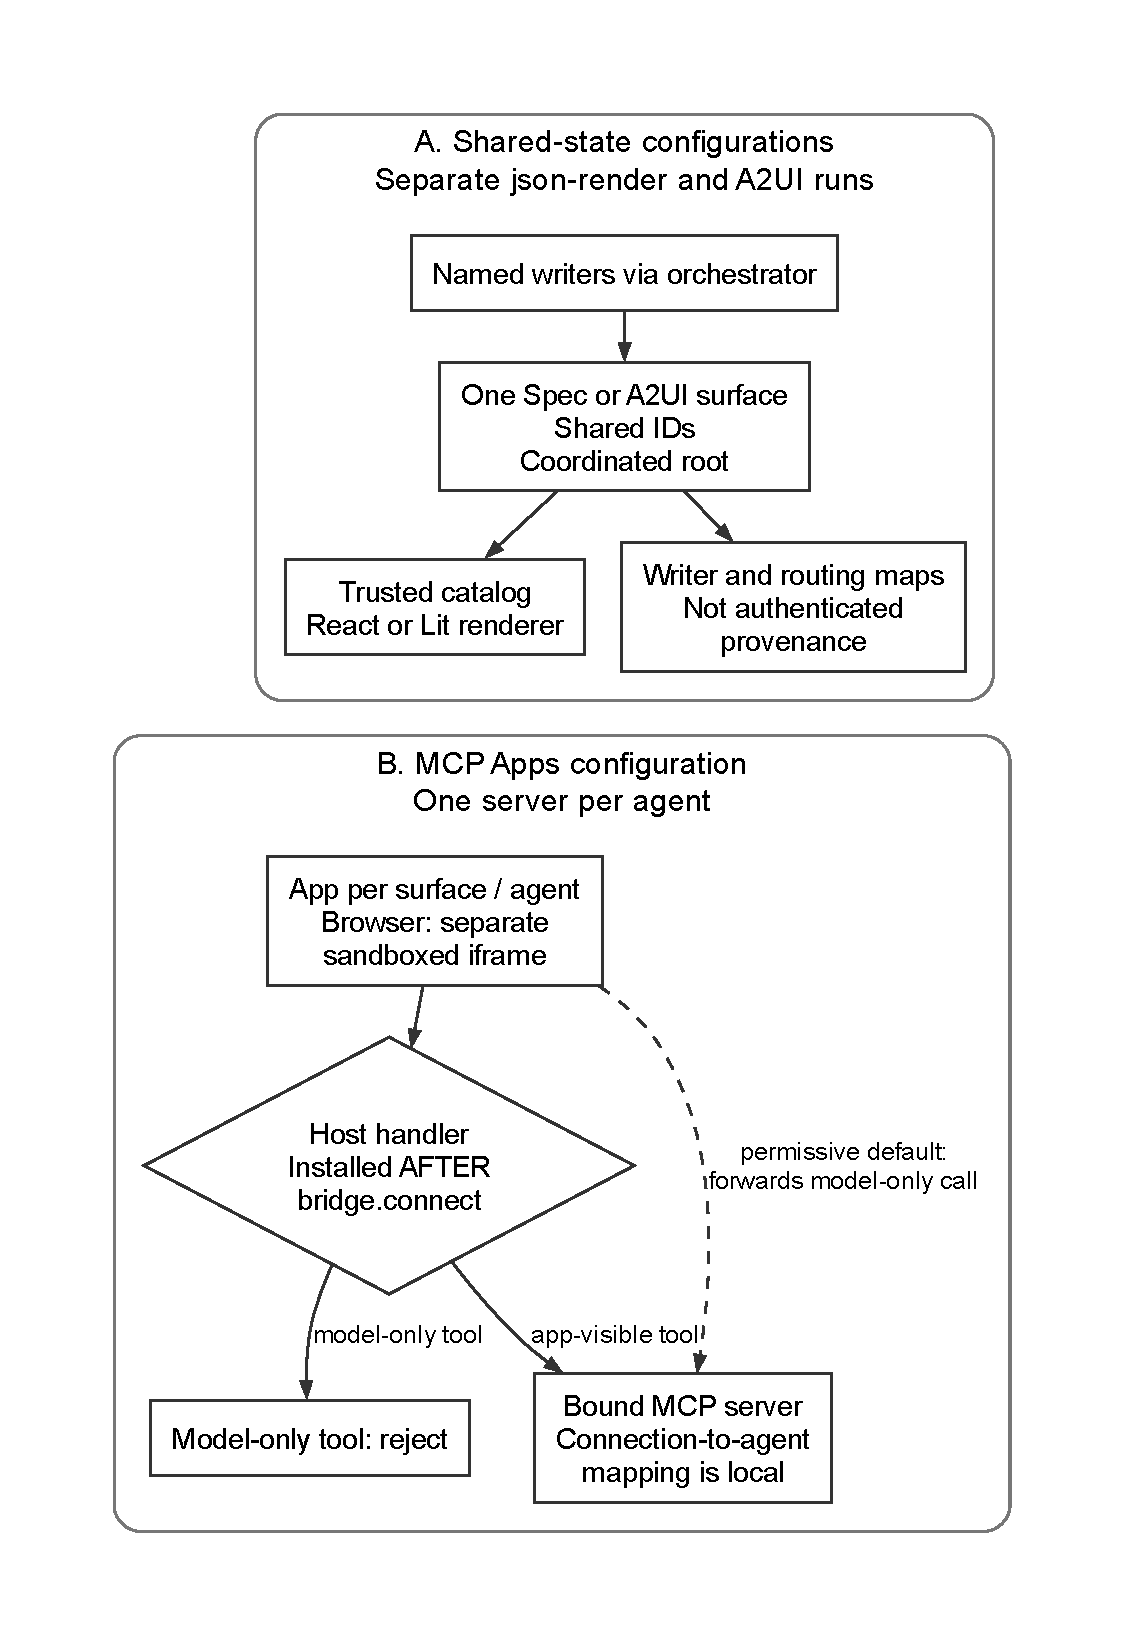
\includegraphics[width=\linewidth,height=0.70\textheight,keepaspectratio]{./figures/topology.pdf}
\caption{Configured state and enforcement boundaries. Panel A summarizes two
separate declarative-renderer runs; panel B shows the app-to-server call
path for each MCP instance. Writer maps are bookkeeping. Only the
installed host handler rejects the model-only call; the permissive
default forwards it. Original source-derived illustration, not a fresh
browser observation.}\label{fig:topology}
\end{figure}

\subsection{Scenario design and evidence
collection}\label{scenario-design-and-evidence-collection}

S1 opens a trip surface, emits a planner itinerary, hands off to
booking, and emits a reservation. S2 performs the fixed-order writes
specified in H1. S3 emits basket and payment controls and activates
ordinary and privileged actions. The amounts and booking operations are
fixtures: the MCP server records calls and returns text; it does not
charge money. The three scenarios are fixed examples, not a sample drawn
from a population of agent workflows.

The \href{../src/scenarios/run.ts}{runner} constructs fresh adapters per
scenario and configuration. The
\href{../src/orchestrator/orchestrator.ts}{orchestrator} is a scripted
stand-in with named agents and a control-to-agent routing table, not an
autonomous model-driven system. We inspect the existing tests and rerun
them where local prerequisites permit; no scenarios or adapters are
added or modified.

The \href{../src/report/generate.ts}{report generator} takes
adapter-authored classifications and uses first-recording-wins selection
for each capability and configuration. It does not independently measure
the meaning of \texttt{SUPPORTED}, \texttt{LOST}, \texttt{ENFORCED}, or
\texttt{NOT\_EXPRESSIBLE}. Repeated labels do not constitute independent
observations. Timestamp normalization makes its Markdown stable but does
not validate its interpretation. A freshness check establishes
correspondence between report and generator, not the truth of every
sentence in the report.

We therefore distinguish classifications from assertions on snapshots,
messages, tool responses/refusals, and rendered elements. The
\href{../tests/protocol/conformance.test.ts}{conformance tests} validate
the S1 A2UI messages and json-render catalog output, examine recorded
patches, and check report and image-link freshness. They do not
establish full specification conformance. The A2UI deletion message is
not exercised in that S1 check. The json-render patch assertions do not
cover its direct root mutation.

Browser evidence has an additional qualification: the MCP browser host
contains its own fixture script. In S2 it renders the two summaries
without the two uncontested detail blocks used by the Node scenario. Its
DOM assertions are useful corroboration for those summaries, not
byte-identical replay of the Node runner. Retained screenshots alone
cannot establish that a fresh browser run passed.

\section{Bounded observed results}\label{bounded-observed-results}

\subsection{RQ1: Handoff and placement}\label{rq1-handoff-and-placement}

Existing S1 assertions check a single \texttt{trip} snapshot region
containing both \texttt{itinerary} and \texttt{reservation} in
json-render and A2UI. MCP Apps checks separate \texttt{trip::planner}
and \texttt{trip::booking} regions. The browser assertions check both
blocks within one React tree or A2UI surface, and separate MCP iframes.
These checks support a placement observation under the chosen mappings.
They do not prove that MCP Apps cannot represent an aggregated UI or
that either declarative format provides authenticated cross-agent
ownership.

\subsection{RQ2: Fixed-order identifier
collision}\label{rq2-fixed-order-identifier-collision}

The focused local S2 rerun passed its three selected tests; ten non-S2
tests in that file were skipped by the filter. The json-render assertion
checks the finance writer and headline, plus survival of the two
uncontested blocks. The A2UI Node assertion checks the finance writer
from adapter bookkeeping; its browser assertion checks headline text.
MCP snapshot assertions check both headlines in different instances. H1
is supported by these local assertions to their respective extent;
A2UI's Node writer field is weaker evidence than a rendered headline.
Fresh browser execution was blocked before tests could run because the
preview server could not listen inside the sandbox. We therefore do not
count its DOM expectations as newly executed evidence.

The replacement is consistent with reusing a slot in these shared
namespaces. It is not an observed scheduling race. The absence of a
protocol-level conflict notification in this script does not mean the
harness is blind to replacement: the adapter itself detects a changed
writer and records it. Namespacing, ownership checks, arbitration, or
shared aggregation could change the outcome; none is evaluated as an
intervention here.

Figure \ref{fig:s2} separates the four awaited writes from the retained
summary states. The arrows express script order, not elapsed time or
competing schedules.

\begin{figure}[!htbp]
\centering
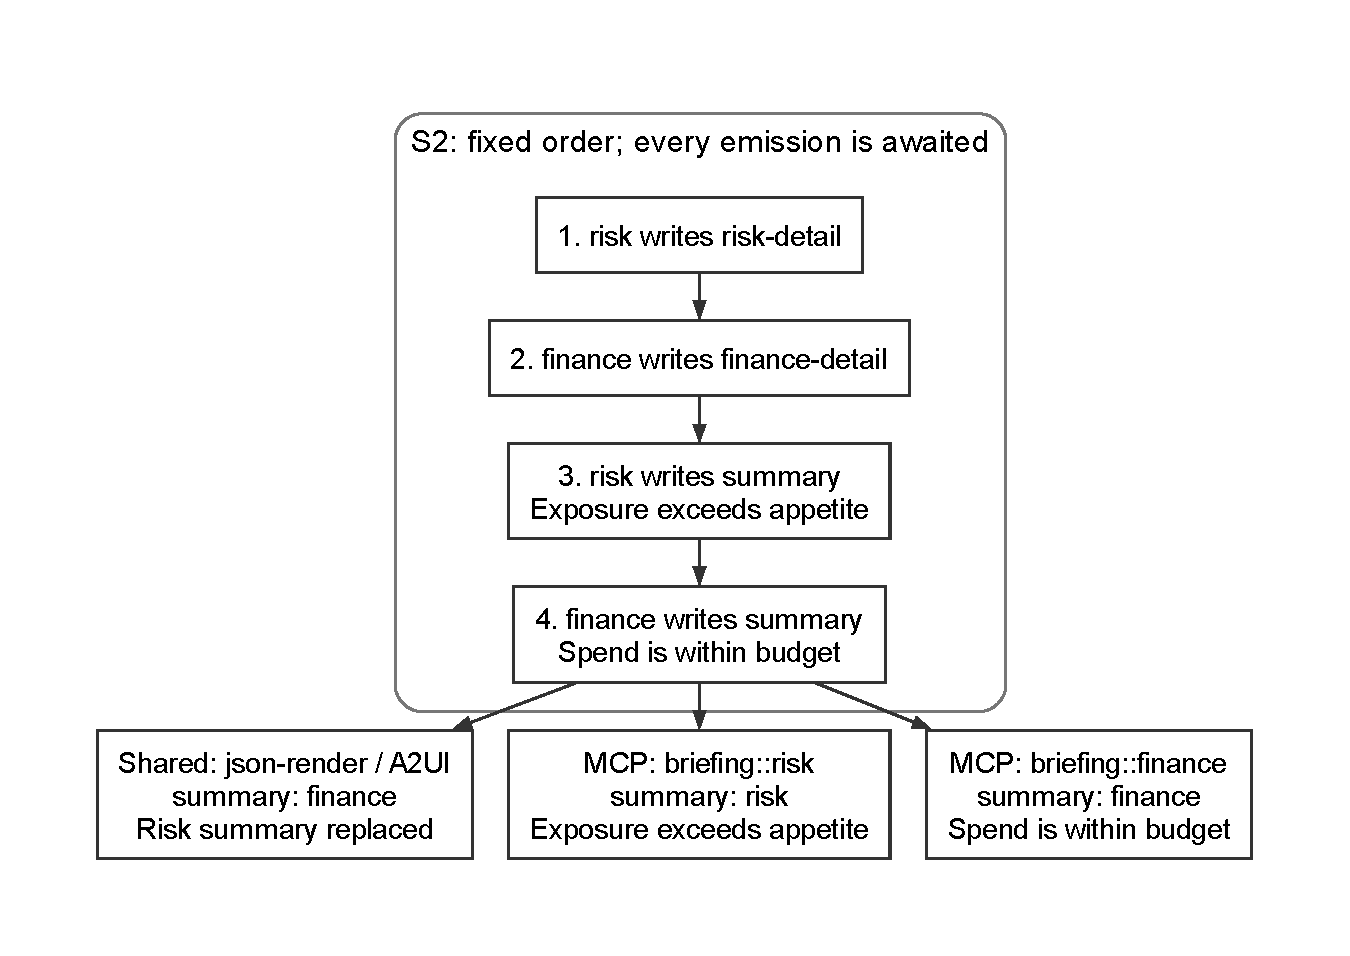
\includegraphics[width=\linewidth,height=0.70\textheight,keepaspectratio]{./figures/s2.pdf}
\caption{S2 write order and retained summaries in the configured namespaces. The
uncontested detail writes precede the collision. Node assertions check
the json-render headline and both MCP headlines; A2UI's Node check
verifies the last-writer map, while its headline DOM assertion remains
unexecuted locally. The two MCP summaries belong to separate instances,
not a merged surface.}\label{fig:s2}
\end{figure}

\subsection{RQ3: Routing and host
decisions}\label{rq3-routing-and-host-decisions}

In the shared-state configurations, ordinary action routing uses the
orchestrator's control table. Tests inspect routing entries and
deliveries, and the A2UI action envelope carries surface/component
fields and a timestamp without an agent field. These payload
observations do not rule out an application-supplied identity envelope.
Encoding a name in context or props would still require trusted binding
before it could authorize anything.

json-render's privileged control includes \texttt{confirm} metadata. The
Node adapter constructs an event and classifies that metadata; it does
not run an independent authorization service. The browser suite clicks
the ordinary json-render action, not the privileged confirmation flow.
Confirmation UI is not independent authorization, and the existing
assertions do not establish complete consent behavior or protection
against an omitted confirmation binding. A2UI has no privileged gate
implemented in this adapter; that is not a proof that its hosts or
trusted catalog components cannot impose one.

For MCP Apps, the \href{../src/adapters/mcp-apps/host.ts}{host} installs
its enforcing \texttt{oncalltool} handler after \texttt{bridge.connect}.
The handler looks up the tool and rejects model-only visibility. The
\href{../tests/protocol/mcp-apps-bridge.test.ts}{bridge tests} check
successful app-visible calls, rejection messages and refusal records,
and successful model-only calls when enforcement is disabled. The
permissive host variant forwards that call. This is evidence about the
tested SDK and handler installation order, not every MCP host or SDK
release. The inspected extension specification assigns visibility
enforcement to the host {[}R4{]}.

Routing evidence is narrower than some trace labels suggest. For
actions, the Node MCP adapter selects the first instance for a
conceptual surface. Its helper is \texttt{findInstanceForSurface}. It
does not find the agent owning the clicked control. The routing test
only requires some delivery without the fallback table. Thus it cannot
prove correct owner routing for every S3 control. Browser S3 instead
clicks inside the cart and payments frames separately. We retain this
distinction and leave the existing behavior unchanged.

\section{Claim-evidence mapping}\label{claim-evidence-mapping}

Here \textbf{supported} means a bounded statement has a matching
inspected assertion or direct source observation, with run status
separately recorded. \textbf{Partial} means a relevant assertion exists
but leaves a material inference untested. \textbf{Proposed} means a
future check has not been performed. These terms are this paper's
evidence statuses, distinct from the adapter outcome vocabulary.

{\def\LTcaptype{none} % do not increment counter
\begin{longtable}[]{@{}
  >{\raggedright\arraybackslash}p{0.3800\dimexpr\linewidth-4\tabcolsep\relax}
  >{\raggedright\arraybackslash}p{0.1400\dimexpr\linewidth-4\tabcolsep\relax}
  >{\raggedright\arraybackslash}p{0.4800\dimexpr\linewidth-4\tabcolsep\relax}@{}}
\toprule\noalign{}
\begin{minipage}[b]{\linewidth}\raggedright
Claim
\end{minipage} & \begin{minipage}[b]{\linewidth}\raggedright
Status
\end{minipage} & \begin{minipage}[b]{\linewidth}\raggedright
Evidence and falsifier
\end{minipage} \\
\midrule\noalign{}
\endhead
\bottomrule\noalign{}
\endlastfoot
C1: S1 yields one shared region or two MCP instances in this topology. &
Supported & S1 snapshot region and block assertions; contradicted by
missing blocks or different region counts. \\
C2: S2 overwrites the json-render summary and retains both MCP
summaries. & Supported & S2 headline assertions; contradicted by
different retained values. \\
C3: S2's A2UI shared summary displays finance's headline. & Partial &
Node checks adapter writer; browser checks rendered value. Fresh DOM
execution remains a separate prerequisite. \\
C4: S2 is sequential, with no scheduling test. & Supported & Four
awaited emissions in the S2 source; contradicted by an overlapping
scheduler in the executed path. \\
C5: The enforcing MCP handler rejects the model-only call, while the
permissive variant forwards it. & Supported & Bridge rejection/refusal
and successful-result assertions; contradicted by reversed or identical
behavior. \\
C6: Every MCP S3 control reaches its intended agent. & Partial &
Existing test checks some table-free delivery; first-instance selection
prevents this stronger inference. \\
C7: json-render includes confirmation metadata, with consent enforcement
incompletely checked. & Partial & Existing check records metadata, not
independent policy or privileged browser consent. \\
C8: Matrix labels are adapter classifications, not independent
measurements. & Supported & Source shows first-recording-wins selection;
freshness checks correspondence only. \\
C9: A matched-topology intervention isolates protocol causality. &
Proposed & Pending controlled comparison; no new experiment is
reported. \\
\end{longtable}
}

The linked scenario, bridge, conformance, and browser test files in
Methodology and Results are the check locations for C1--C8. This mapping
exposes uneven coverage rather than assigning a numeric score across
unlike checks.

\section{Related work}\label{related-work}

The json-render repository describes catalog-defined components and
actions rendered from structured specifications {[}R1{]}. A2UI similarly
separates declarative UI data from client implementation and describes a
trusted component catalog {[}R2{]}. These are meaningful security
properties: constraining requested components and handlers can limit
what untrusted UI data asks the client to run. They do not by themselves
establish per-writer authorization in our shared namespace. Conversely,
our collision example is not evidence of blanket insecurity in
declarative rendering.

The MCP Apps repository describes tool-associated UI resources and a
host bridge {[}R3{]}. Its specification describes visibility checks and
sandbox/CSP obligations {[}R4{]}. Those obligations are not proof that
this harness checks all of them. In particular, iframe sandbox
attributes and successful bridge tests do not establish exhaustive CSP
enforcement, transport security, or resistance to malicious content.
Declarative catalogs and sandboxed app delivery are compatible layers: a
hosted application could use a declarative renderer internally. No
integration experiment is reported here.

The requested methodological reference is
\href{https://github.com/besanson/sarc-authority-derivation}{besanson/sarc-authority-derivation}.
Access attempts for its README, REPRODUCTION.md, NOVELTY.md, and paper
directory failed in this environment. We attribute the intended
methodological influence explicitly, but cannot claim direct inspection
of its manuscript or verification of its results. The user's description
of that project's practices motivated our research questions, claim
table, status vocabulary, and execution ledger. No prose or scientific
results from that project are used as evidence here. Any reproduction
credited there to Eduardo concerns that project only. The present work
is neither replication of it nor an independent-person reproduction. The
reference inspection remains pending, and this related-work discussion
is deliberately selective rather than an exhaustive literature or
novelty review.

\section{Threats to validity}\label{threats-to-validity}

\textbf{Internal validity.} Identical logical inputs leave adapter
bookkeeping, shared-root coordination, naming conventions, host
enforcement, catalogs, rendering frameworks, transports, and
one-server-per-agent MCP topology as confounders. The default/permissive
MCP comparison narrows one host-policy question, but it is not a
factorial comparison across all configurations.

\textbf{Construct validity.} A region count is a property of the adapter
snapshot; it is not a usability measure. A writer prop is not
authenticated provenance. Addressability is not authority. A
confirmation binding is not an authorization decision. Adapter labels
and some scenario assertions share their interpretation, creating a risk
of circular validation. The independent aspects of the checks are the
inspected contents, response/refusal assertions, and DOM expectations;
they are still authored within this repository, not by independent
evaluators.

\textbf{Execution and coverage.} Node transports do not test browser
isolation. The MCP browser fixtures differ from the Node scenario.
Existing screenshots are retained artifacts with no newly established
capture provenance. The suite does not comprehensively test adversarial
inputs, identity forgery, transport authentication, CSP, cross-server
policy, authorization revocation, or arbitrary concurrent schedules. No
completed security review is claimed.

\textbf{External and temporal validity.} Three designed scenarios, fixed
fixture data, and the pinned installed packages cannot establish
population effects or general protocol superiority. Later SDKs, other
renderers, different server topologies, and stricter application
policies can behave differently. Mutable upstream documentation is
contextual evidence, not a version-pinned release archive. No latency,
throughput, cost, user study, or model capability was measured.

\section{Reproducibility}\label{reproducibility}

The \href{./REPRODUCTION.md}{reproduction guide} gives commands and
expected semantic outcomes. The \href{./EXECUTION.md}{local execution
record} separates successful commands, failures, unavailable
prerequisites, and retained artifacts. The base revision is
\texttt{b895e57671e118fcd3a7f86892fc1b2526b78c9c}; the initial working
tree was clean. The manuscript, generated derivatives, checks, and
documentation additions are local uncommitted work on that base. Neither
the historical revision supplied as a hint nor a clean base revision
alone identifies the final paper workspace. The execution record and
file hashes identify the relevant inputs and outputs.

Semantic reproducibility means obtaining the specified regions, values,
events, and refusal behavior under the same configuration. Byte identity
is a separate question. A2UI action timestamps vary; report generation
normalizes those timestamps. PDF metadata and toolchain resources can
also vary. We check generated LaTeX against fresh Pandoc output under
the recorded toolchain, not PDF byte identity across machines. The
Markdown manuscript is the only editable paper source; LaTeX and PDF are
generated derivatives.

This session is an agent-assisted local rerun of existing checks. It
establishes neither independent-person reproduction nor human approval.
The previous session's reported dependency installation is not a fresh
\texttt{npm\ ci} execution in this record. Missing checks and failed
attempts remain visible rather than being counted as passes. OpenSpec
command success cannot prove every acceptance criterion.

The complete local Vitest run passed 24 tests across three files and
TypeScript checking passed. The standalone \texttt{report:check} command
failed when tsx attempted to create an IPC listener (\texttt{EPERM});
the report freshness assertion inside the passing Vitest suite is
separate evidence, not a successful standalone command. The browser
command built the pages but failed to start its preview server
(\texttt{EPERM} on \texttt{::1:5178}), so no fresh browser test success
is claimed. Pandoc produced LaTeX and its freshness check passed. The
initial Tectonic invocation panicked internally (exit 101) in
cached-only mode. A later local build used an explicit directory bundle
assembled from already cached TeX resources and a smaller template, and
produced the illustrated PDF without network access or shell escape.
Original Mermaid diagrams were converted locally to vector figures
through a restricted Mermaid-to-Graphviz renderer after Chromium-based
rendering failed. These illustrations explain source and assertions;
they add no experiments. The execution record retains the historical
failures and current inspection evidence. Local compilation does not
establish arXiv TeX Live compatibility or publication acceptance. Human
review remains pending.

\section{Conclusion}\label{conclusion}

For the inspected configurations, handoff placement and repeated
identifiers follow the chosen shared or separated namespaces, while MCP
model-only tool rejection depends on the enforcing host handler. The
strongest local conclusion is that claims must name the adapter mapping
and enforcement site alongside the SDK or protocol. The results do not
establish unavoidable incompatibility between composition and security.
Integrations remain possible, and trusted catalogs remain relevant
security mechanisms.

Future experiments are explicitly pending: matched namespaces and
topology, controlled scheduling with overlapping writes, trusted
identity envelopes, privileged confirmation interaction tests, and
complete host-policy tests. They are suggestions for separate approved
work, not results of this paper.

\section{AI-assistance disclosure}\label{ai-assistance-disclosure}

Eduardo Arana (Arananet) is the named author at the user's request. An
OpenAI Codex coding assistant inspected source and available references,
drafted this English manuscript and supporting documentation, added
focused checks, and executed local validation commands. This disclosure
does not assert that Eduardo personally performed each command, reviewed
every claim, or approved publication. Human review pending: the author
must assess scientific accuracy, citations, limitations, and final
presentation. AI-assisted drafting is separate from the deterministic
harness: no LLM participates in its scenario experiments. No model
identifier is inferred from an invocation request or catalog
description.

\section{References}\label{references}

R1. Vercel Labs.
\href{https://github.com/vercel-labs/json-render}{json-render repository
and README}. Inspected 21 September 2026; live main, upstream commit not
retained. Local SDK context: \texttt{@json-render/core} and
\texttt{@json-render/react} 0.21.0, including the installed core README
and manifest. Used for catalog/renderer design, not a security proof.

R2. A2UI project. \href{https://github.com/a2ui-project/a2ui}{A2UI
repository and README} (the inspected \texttt{google/A2UI} URL redirects
here). Inspected 21 September 2026; live main, upstream commit not
retained. Local context: web core and Lit 0.11.0, installed web-core
README, and adapter-selected v0.9 schema.

R3. Model Context Protocol contributors.
\href{https://github.com/modelcontextprotocol/ext-apps}{MCP Apps SDK
repository and README}. Inspected 21 September 2026; live main, upstream
commit not retained. Local context: extension, client, core, and server
packages 2.0.0; extension README and manifests inspected. SDK package
version is distinct from wire version.

R4. Model Context Protocol contributors.
\href{https://github.com/modelcontextprotocol/ext-apps/blob/main/specification/draft/apps.mdx}{MCP
Apps extension specification, draft/apps.mdx}. Visibility and
sandbox/CSP sections inspected 21 September 2026; mutable main path, no
pinned specification commit. Used to distinguish host requirements from
the assertions implemented here. The filename's ``draft'' is retained as
the source location, without claiming a release status from the SDK
version.
\end{document}
